
\documentclass{IOS-Book-Article}
\usepackage{graphicx}

\usepackage{float} % keeps tables in the exact position they occupy in the code
\usepackage{mathptmx}
\usepackage{soul}\setuldepth{article}
%\usepackage{times}
%\normalfont
%\usepackage[T1]{fontenc}
%\usepackage[mtplusscr,mtbold]{mathtime}
%
\def\hb{\hbox to 11.5 cm{}}

\begin{document}

\pagestyle{headings}
\def\thepage{}
\begin{frontmatter}              % The preamble begins here.


%\pretitle{Pretitle}
\title{Health-related content in Transformer-based language models.}

\markboth{}{January 2023\hb}
\subtitle{Exploring bias in domain general vs. domain specific training sets.}

\vspace{-4mm}
\author[A]{\fnms{Caterina} \snm{Bonan}\orcid{0000-0002-4808-6865}%
}
and
\author[B]{\fnms{Giuseppe} \snm{Samo}\orcid{0000-0003-3449-8006}
\thanks{Corresponding Author: Giuseppe Samo, Department of Linguistics, University of Geneva, E-mail: giuseppe.samo@unige.ch; mail: Rue de Candolle 2, 1205 Geneva, Switzerland. }}
\runningauthor{Bonan \& Samo}
\address[A]{University of Cambridge}
\address[B]{University of Geneva}

\begin{abstract}
In this communication, we demonstrate that the bias observed in domain general training sets with health-related content is not improved in domain specific health-communication corpora, \textit{contra} \cite{r1}.
\end{abstract}

\begin{keyword}
Natural Language Processing\sep Health-content\sep 
Language Models\sep Knowledge Reproduction\sep Corpora\sep COVID-19
\end{keyword}
\end{frontmatter}
\markboth{January 2023\hb}{January 2023\hb}
%\thispagestyle{empty}
%\pagestyle{empty}

\vspace{-6mm}
\section{Introduction}

%aggiungere articolo della Ettinger
Artificial neural language models (LMs) parse and generate complex linguistic structures across languages \cite{r2}, and can be used for fact checking \cite{r3}. 
In \cite{r1}, we detected syntactic bias in Transformer-based LMs using a list of myth busters on COVID-19 from parallel World Health Organization corpora. We demonstrated that when LMs are queried with sentences compared with \textit{ad hoc} examples with opposite polarity, asymmetries are easily detected and quantified.
Here, we explore six training sets for English and Chinese LMs to detect bias with respect to domain-specific (i.e., medical) semantico-encyclopedic knowledge, adopting and improving the dataset previously discussed in \cite{r1}.\footnote{Information on the data is available at the following link:\href{https://github.com/samo-g/health-transformer}{\underline{https://github.com/samo-g/health-transformer}}.}

\vspace{-4mm}
\section{The study}
\textbf{Hypothesis} In \cite{r1}'s conclusions, we tentatively attributed the observed bias to the type of training data under investigation, and hypothesised that LMs trained on domain specific datasets might perform better than those trained with domain general data.

\noindent \textbf{Materials} The queried parallel datasets for English and Chinese are those presented in \cite{r1}. The training sets for this contribution are presented in table \ref{models}.

\begin{table}[]
    \centering
    \begin{tabular}{l|l|l}
          & \textsc{Training set type} & \textsc{Language Models}\\ \hline
         \textsc{English} & Domain general (web, wiki) & \href{https://huggingface.co/bert-large-cased}{\underline{BERT}}, \href{https://huggingface.co/google/bigbird-pegasus-large-pubmed}{\underline{BigBird}}\\
         & Domain specific & \href{https://huggingface.co/austinmw/distilbert-base-uncased-finetuned-health_facts}{\underline{HealthF}} (fact checking), \href{https://huggingface.co/publichealthsurveillance/PHS-BERT}{\underline{PHS}} (health surveillance on social media)\\ \hline
         \textsc{Chinese} & Domain general (web, wiki) & \href{https://huggingface.co/bert-base-chinese}{\underline{Bert}}\\
         & Domain specific & \href{https://huggingface.co/nghuyong/ernie-health-zh}{\underline{HealthZH}} (medical dialogues, records, textbooks)\\ \hline
    \end{tabular}
    \caption{Language Models used in this paper. All references are available as hyperlinks.}
    \label{models}
\end{table}

\noindent \textbf{Methods} As in \cite{r1}, the machine is presented with two sentences: (i) a \textsc{true} statement from the corpus and (ii) a \textsc{false} counterpart created using logical operators. Our measure is represented by the difference between the surprisal of the \textsc{true} and the \textsc{false} statement. The surprisal is the logarithm of the reciprocal of the output probability in a fill-mask task. In a nutshell, lower surprisal is to be expected for \textsc{true} sentences.

\begin{figure}
    \centering
    \small
    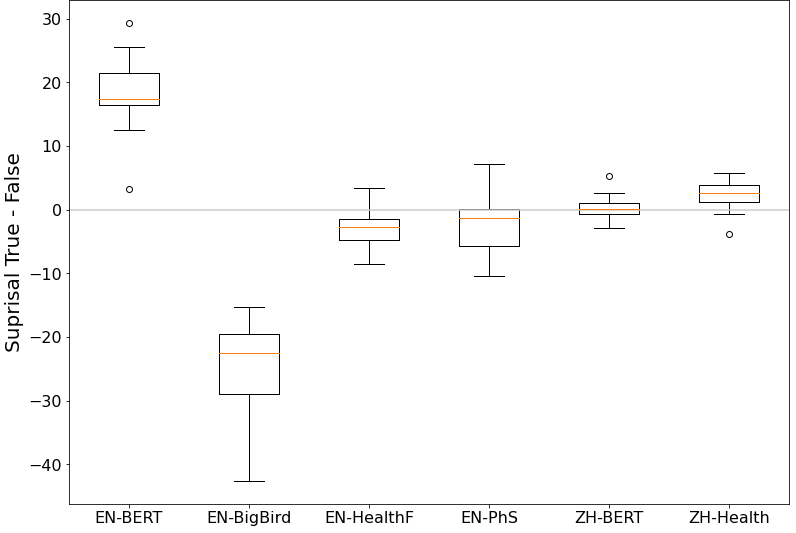
\includegraphics[scale=0.37]{graphmatplot}
    \caption{True-False across language models. }
    \label{results}
\end{figure}

\noindent \textbf{Results} Figure \ref{results} displays an asymmetry for English (\textit{F}(3, 64) = 177.30362; p $<$ .00001): while the BERT general domain LM performs worse (\textit{M} = 18.269, \textit{SD = 5.82}) than domain specific ones, BigBird (\textit{M} = -24.459, \textit{SD} = 7.0771364) shows the least surprisal on \textsc{true} statements, plausibly due to its architecture combining sparse and global attention. In Chinese, the general domain performs better (\textit{M} = 0.510, \textit{SD} = 2.421) than the domain-specific one (\textit{M} = 1.81, \textit{SD} = 2.418) (\textit{t}(34) = 2.6837, p. $<$ .05).

\vspace{-4mm}
\section{Conclusions}
\cite{r1} provided a methodology for the detection of bias in LMs that can be adopted to fact checking and the general medical domain, and predicted lower bias with health-specific training sets. Here, we showed that domain specific training sets do not necessarily perform better than domain general ones. Future studies should explore additional datasets (e.g., online medical training, \cite{r4}) and languages.

\vspace{-4mm}
\begin{thebibliography}{99}


\bibitem{r1}
Samo G, Bonan C, Si F. Health-Related Content in Transformer-Based Deep Neural Network Language Models: Exploring Cross-Linguistic Syntactic Bias. Stud Health Technol Inform. 2022 Jun 29;295:221-225. doi: 10.3233/SHTI220702. PMID: 35773848.

\bibitem{r2}
Linzen T, Baroni M. Syntactic Structure from Deep Learning. Annual Review of Linguistics 7:1,
Jan.2021;195-212.

\bibitem{r3}
Ahmed S, Hinkelmann K, Corradini F, Development of fake news model using machine learning through natural language processing; arXiv:2201.07489, Jan. 2022. 
  

\bibitem{r4}
Utunen H, Ndiaye N, Piroux C, George R, Attias M, Gamhewage G, Global Reach of an Online COVID-
19 Course in Multiple Languages on OpenWHO in the First Quarter of 2020: Analysis of Platform Use
Data, J Med Internet Res. 22 (2020) e19076. doi:10.2196/19076.

\end{thebibliography}
\end{document}